\paragraph{Bochner-Ries summability}
Q: In which way does Fourier inversion hold? (In $L^p(ℝ^d)$)
\[f(x)=∫_{ℝ^d}\hat f(ξ)e^{2πixξ}\mdξ=\lim_{R→∞}\underbrace{∫_{|ξ|<R}\hat f(ξ)(1-\frac{|ξ|^2}{R^2})^δe^{2πixξ}\mdξ}_{f*k_δ}?\]
for suitable $δ\geq 0$.
\[δ>\frac{d-1}2⇒k_δ∈L^1(ℝ^d)\]
\[δ\leq \frac{d-1}2\qquad δ=0\text {today}\]
$d=1$: The second equality holds in $L^p$-norm ($1<p<∞$) $\impliedby L^p$ boundedness of Hilbert transform

and also a.e.\ $(p=2$ Carleson '66 $1<p<∞$ Hunt '68)

$d\geq 2$ Let us only consider norm convergence
\[f↦(S^δf)(x)=∫_{|ξ|\leq 1}\hat f(ξ)(1-|ξ|^2)^δe^{2πixξ}\md ξ\]
\[Sf(x)=∫_{|ξ|\leq 1}\hat f(ξ)e^{2πixξ}\mdξ\]
\[\hat{Sf}=1_{|ξ|\leq 1}\hat f\]
($\hat{Hf}=iπ\sgnξ\hat f$)
\[\|Sf\|_{L^2(ℝ^d)}=\|\hat{Sf}\|_{L^2}=\|1_{|ξ|\leq 1}\hat f\|_{L^2}\leq\|\hat f\|_{L^2}=\|f\|_{L^2}\]
He said something about every bounded operator can be written like this or so? 
Fourier multiplier is bounded iff multiplier is bounded.

\begin{theo}[C.Fefferman '71 -- Annalis of ath. –THe multiplier problem for the ball"]
	Suppose $q\geq 2$ and $p\neq 2$. Then the opertor $S$ (initially defined on $L^p∩L^2$) is not extendable to a bounded operator from $L^p(ℝ^d)$ to itself.
\end{theo}

\begin{proof}
	Let $B⊂ℝ^d$ ball, let $S_B$ be the multiplier orator associated to $B$:
	\[\hat{S_Bf}=1_B\hat f.\]
	Given $u∈S^{d-1}⊂ℝ^d$, let $S^n$ be the multiplier operator associated to the half-space with normal $u$:
	\[\hat{S^uf}=1_{\{ξu>0\}}\hat f\qquad (S^uf)(x)=∫_{ξu>0}\hat f(ξ)e^{2πixξ}\mdξ\]
	Upshot: $L^p$ bound for $S$ implies an $L^p$ vector-valued inequality for $S_B$s and $S_u$s.

	\begin{lem}[Y. Mèyer]%wrong direction
		Suppose \[\|Sf\|_{L^p}\leq A_p\|f\|_{L^p}\]
		$f∈(L^2∩L^p)(ℝ^d)$ holds for some $p∈[1,∞]$. Suppose $f_1,…,f_M∈L^2∩L^p,\ u_1,…,u_M∈S^{d-1}⊂ℝ^d$. Then
		\[\|(\sum_{j=1}^M||S^{u_j}(f_j)|^2)^{\frac12}\|_{L^p(ℝ^d)}\leq A_p\|(\sum_{j=1}^M|f_j|^2)^{\frac12}\|_{L^p(ℝ^d)}\]
		where $A_p$ is the same constant as above.
	\end{lem}
	\begin{proof}[Proof of Lemma]
		Step 1: $B=B_R=$ ball of radius $R$ centered at $0$. Then
		\[\|S_B(g\|_{L^p}\leq A_p\|f\|_{L^p})\quad(g∈L^2∩L^p)\]%(*)
		Why? Scaling: \[δ_R(g)(x)=g(\frac xR)\] Check $δ_{R^{-1}}\circ S\circ δ_R=S_{B_R}$ since $S=S_{B_1}$. $\hat{δ_ρ(g)}(ξ)=R^d\hat g(Rξ)$.

		Step 2: $M$ balls. ($p<∞$) $f=(f_1,…,f_M)$ given $M$-tuple of functions. $T(f):=(Tf_1,…,Tf_M)$. Given a unit vector $ω=(ω_1,…,ω_M)∈ℂ^M$, let
		\[S_ω(f)=\sum_{j=1}^M\barω_jS_B(f_j)=S_B(\sum_j\barω_jf_j)=S_B(f_ω)\quad f_ω=\sum_{j=1}^M\barω_jf_j\]
		\[(*)⇒∫_{ℝ^d}|S_ωf(x)|^p\md x\leq A_p^k∫_{ℝ^d}|f_ω(x)|^p\md x\]%(**)
		$(S_ωf)(x)=?$. $x,y∈ℂ^M$
		\[\langle x,y\rangle=\sum_{i=1}^Mx_j\bar y_j\]
		\[S_ω(f)(x)=S_B(f_ω)(x)=S_B(\sum_{j=1}^M\barω_jf_j)(x)=\sum_{j=1}^M\barω_jS_B(f_j)(x)|=|\langle S_B(f)(x),ω\rangle|=|S_B(f)(x)||\langle\frac{S_B(f)(x)}{|S_B(f)(x)|},ω,\rangle|=(\sum_{j=1}^M|S_B(f_j)(x)|^2)^{\frac12}|φ(ω,S_B(f)(x))|\]
		Integrate both sides of (**) with respect to $ω$ (before integrating in $x$).
		\[\text{LHS}=∫_{ℝ^d}(∫_{|ω|=1}|S_ω(f)(x)|^p\mdω)\md x=∫_{ℝ^d}(\sum_{j=1}^M|S_B(f_j)(x)|^2)^{\frac p2}\underbrace{(∫_{|ω|=1}|Φ(ω,S_B(f)(x)|^p\mdω)\md x)}_{0\neq γ_p=∫_{|ω|=1}|Φ(ω,1)|^p\mdω})\md x\]
		For fixed $ν∈S^{d-1}$ $∫_{S^{d-1}}|\langleω,ν\rangle|^p\mdσ_ω=ω_{d-2}∫_{-1}^1(1-t^2)^{\frac{d-3}2}\md t$.

		Similarly,
		\[\text{RHS}=∫_{ℝ^d}(\sum_{j=1}^M|f_j(x)^2)^{\frac p2}\md x)γ_p\]
		\[(**)⇒\|(\sum_{j=1}^M|S_B(f_j)|^2)^{\frac12}\|_{L^p(ℝ^d)}\leq A_p\|(\sum_{j=1}^M|f_j|^2)^{\frac12}\|_{L^p(ℝ^d)}\]

		Step 3: From balls to half-spaces

		$B_R^u=$ ball of radius $R$ centered at $Ru$. Upshot: $B_R^u→\{ξu>0\}$ as $R→∞$. 

		Translation:
		\[(TVjf)(x)=f(x-y)\]
		\[\hat{T_jf}(ξ)=e^{iξy}\hat f(ξ)\]
		\[S_{B_R^u}(f)(x)=e^{2πiuRx}S_{B_R}(fe^{-2πiuRx})\]
		(***) implies
		\[\|(\sum|S_{B_R^{u_j}}(f_j)|^2)^{\frac12}\|_{L^p}\leq A_p\|(\sum|f_j|^2)^{\frac 12}\|_{L^p}\]
		Let $R→∞$ to finish:
		\[\therefore S_{B_R^{u_j}}(f_j)→S^{u_j}(f_j)\quad R→∞(\text{ in }L^2)\]
		$\therefore$ there exists an almost everywher converging subsequence, done.
	\end{proof}

	$\hat{Sf}=1_{B(0,1)}\hat f$. $S$ is not bounded in $L^p(ℝ^d)$ unless $d=1$ or $p=2$. Focus on multiplieer operator for the half-space ($S^u$), $d=1$.
	\[(S^+f)(x)=∫_0^∞\hat f(ξ)e^{2πixξ}\mdξ\quad(f∈L^2)\]
	\[|(S^+f)(x)|\geq\frac c{|x|}\quad\text{if }|x|\geq12\]
	\begin{proof}
		\[(S^+f)(x)=\lim_{ε→0}∫_0^∞\hat f(ξ)e^{2πi(x+iε)ξ}\mdξ\quad\text{in }L^2\]
		\[∫_{-∞}^∞(∫_0^∞e^{-2πiyξ}e^{2πi(x+iε)ξ}\mdξ)f(y)\md y=\frac1{2πi}∫_{-\frac12}^{\frac12}\frac1{y-x-iε}\md y\]
		This has absolute value $\geq c{|x|}$ if $|x|\geq\frac12$.%simgegq

		Alternative proof: $|H(f)(x)|\geq|x|^{-1}$ for large $x$, $S^+=\frac12(I+iH)$.
		\begin{figure}[H]
			\centering
			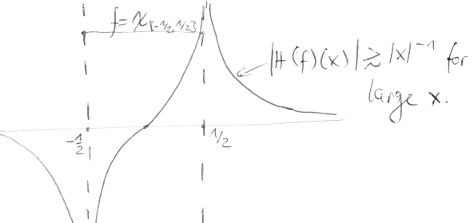
\includegraphics{lec10_01}
		\end{figure}
	\end{proof}
	\begin{figure}[H]
		\centering
		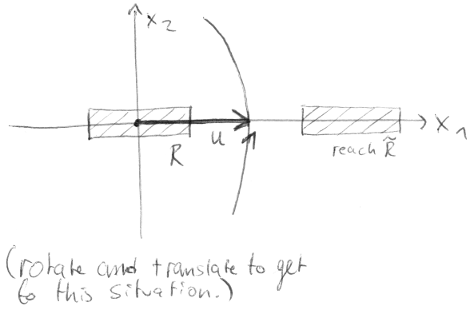
\includegraphics{lec10_02}
	\end{figure}
	$R=(-\frac12,\frac12)\times(-\frac1{2^{N+1}},\frac1{2^{N+1}})$
	\[1_R=1_{(-\frac12,\frac12)}\otimes1_{(-2^{-(N+1)},2^{-(N+1)})}\]
	If $u$ points in the direction of $x_1$ then
	\[(S^u1_R)(x_1,x_2)=(S^+1_{(-\frac2,\frac12)})(x_1)1_{(-2^{-(N+1)},2^{-(N+1)})}(x_2)\]
	\[(1)⇒|S^u(1_R)|\geq c'1_{\tilde R}\]
	Similarly for any $1\times 2^{-N}$ rectangle $R_j$. $u_j∈S^1$ in the positive diretcino of the longest side of $R_j$. Rotate and translate, then
	\[\sim|S^{u_j}(1_{R_j})|\geq c'1_{\tilde R_j}\]
	Take $R_1,…,R_{2^N}$ to be the collection given by $ε$-Kakeya construction, plug that into result from lemma, get a contradiction.

	Key: $p<2$ and $d=2$.

	Lemma with $f_j=1_{R_j}$ and $M=2^N$
	\[c'\underbrace{\leq}_{\text{(3),since $\bigcup\tilde R_j|=1$}}\|(\sum_{j=1}^{2^N}|S^{u_j}(1_{R_j})|^2)^{\frac12}\|_{L^p(ℝ^2)}\leq A_p\|(\sum_{j=1}^{2^N}|1_{R_j}|^2)^{\frac12}\|_{L^p(ℝ^2)}=A_p(∫_E(\sum_{j=1}^{2^N}|1_{R_j}|^2)^{\frac12}\md x)^{\frac1p}\leq A_pε^{\frac1{pq}>0\text{ bc }p<2}\]

	\[\text{smth}\leq|E|^{\frac1q}(∫(\sum|1_{R_j}|^2)^{\frac p2\frac2p}\md x)^{\frac1p\frac p2}=\sum_{j=1}^{2^N}|R_j|=1\]
	\[E=\bigcup_{j=1}^{2^N}R_j\quad |E|<ε,\quad \frac1q+1{2/p}=1,\quad \frac1q=1-\frac p2,\quad\frac1{pq}=\frac1p(1-\frac p2)\]
	Hölder somewhere

	Let $ε<0^+$ to finish

	$d>2$:
	\[f_j(x∈ℝ^d)=f_j(x_1,x_2,x∈ℝ^{d-2})=1_{R_j}(x_1,x_2)f(x')\quad f∈S(ℝ^{d-2})\]
	$p>2$:
	\[\langle Sf,g\rangle=\langle\hat{Sf},\hat g\rangle=\langle 1_B\hat f,\hat g\rangle=\langle \hat f,1_B\hat g\rangle=\langle f,Sg\rangle\quad S=S^*\]
\end{proof}
